\documentclass{article}
\usepackage{fullpage}
\usepackage[czech]{babel}
\usepackage{amsfonts}
\usepackage{amsmath}
\usepackage{graphicx}
\usepackage{caption}
\graphicspath{{images/}}

\title{\vspace{-2cm}Fyzika druháku\vspace{-1.7cm}}
\date{}
\author{}

\begin{document}
\maketitle

\part{Struktura pevných látek}

\section{Krysatlografické soustavy}
AAAAAAA

\section{Deformace}

  \begin{minipage}{0.25\textwidth}\raggedleft
    \begin{itemize}
      \item typy:
      \begin{itemize}
        \item tahem/tlakem
        \item kroucením
        \item ohybem
        \item smykem
      \end{itemize}
    \end{itemize}
  \end{minipage}
  \hspace{0.5cm}
  \noindent\begin{minipage}{0.12\textwidth}
    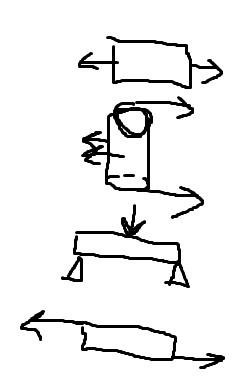
\includegraphics[width=0.9\linewidth]{deformace}
  \end{minipage}

  \section{Deformace tahem/tlakem}

    \begin{itemize}
      \item Normálové nápětí:
      	\begin{equation*}
          \sigma=F/S; [N/m^2] = [Pa]
        \end{equation*}
        \begin{center}
          \vspace{-0.25cm}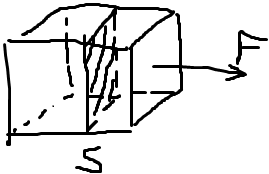
\includegraphics[width=0.12\textwidth]{normalove_napeti}\vspace{-0.25cm}
        \end{center}
      \item Změna délky:
        \begin{equation*}
          \Delta l = l - l_0; \ [m]
        \end{equation*}
      užitečnější většinou relativní prodloužení:
        \begin{equation*}
          \varepsilon = \Delta l/l_0; \ [bezrozm.]
        \end{equation*}
    \end{itemize}

    \subsection{Deformační křivka}
      \begin{center}
        \vspace{-0.1cm}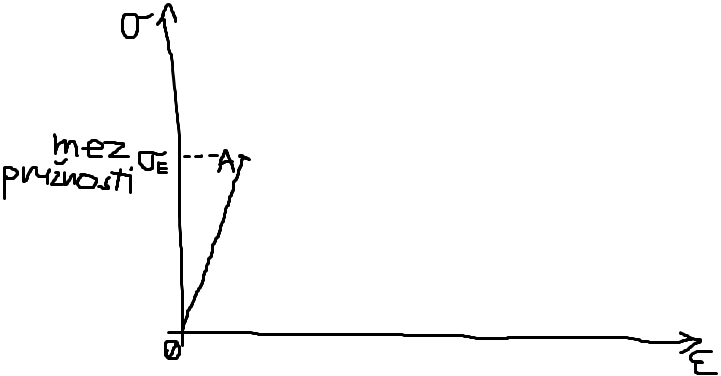
\includegraphics[width=0.75\linewidth]{deformacni_krivka}\vspace{-0.25cm}
      \end{center}

      \begin{itemize}
        \item lineární úsek (0 - A)
        \begin{itemize}
          \item pružná deformace
          \item vratná
          \item platí Hookův zákon:
            \begin{equation*}
              \varepsilon \propto \sigma
            \end{equation*}
          tedy slovy: relativní prodloužení je přímo úměrné napětí (ano, to je symbol pro přímou úměrnost, zapamatujte si ho)
            \begin{equation*}
              \sigma = E*\varepsilon
            \end{equation*}
          E - Youngův modul pružnosti (např. ocel = 220 GPa, cín = 55 GPa, tj. tlak potřebný, abychom objekt roztáhli na dvojnásobnou délku)
        \end{itemize}
        \item nelineární deformace (A - B)
        \begin{itemize}
          \item plastická deformace
          \item protažení bylo dost velké, aby přesunulo atomy v krystalické mřížce na jiné místo
          \item materiál tedy ztráci schopnost se po deformaci vrátit do původního tvaru
          \item při překročení meze pevnosti se materiál prostě trhá na dva kusy
        \end{itemize}
      \end{itemize}

        \subsubsection{Příklady}
        \begin{enumerate}
          \item O kolik se protáhne ocelový drát když na něj zavěsíme závaží:
          \begin{equation*}
            d = 1 mm;
            l = 5 m;
            m = 30 kg;
            E = 220 GPa
          \end{equation*}
          \begin{itemize}
            \item[]
          \end{itemize}
          \begin{equation*}
            \sigma=\frac{F}{S}=\frac{300}{\pi*0,0005^2}
          \end{equation*}
          \begin{equation*}
            \varepsilon = \frac{\sigma}{E}
          \end{equation*}
          \begin{equation*}
            \varepsilon = \frac{F}{S*E}=\frac{\Delta l}{l_0}
          \end{equation*}
          \begin{equation*}
            \Delta l = \frac{F*l*0}{S*E}=8,7*10^{-3} m = 8,7 mm
          \end{equation*}
          \item Na ocelové lanko zavěsíme závaží. Jak těžké může být, aby se lanko nepřetrhlo:
          \begin{equation*}
            d = 1 mm;
            \sigma_p = 1,3 GPa;
            K = 5
          \end{equation*}
          \begin{enumerate}
            \item závaží je v klidu
            \item závaží se hýbe nahoru
            \begin{equation*}
              a = 1 m/s^2
            \end{equation*}
            \item jako kyvadlo OBRAZEKOBRAZEK
          \end{enumerate}
        \end{enumerate}

\part{Změny skupenství}
Př.: OBRAZEKOBRAZEK
$m = 0,2 kg$
a) teplota varu: 50 stupnu
b) c(kap.) $c = Q/(m*deltat)=200/(0,2*40) = 25$ $Jkg^{-1}K^{-1}$
c) c(plyn) $c = Q/(m*deltat)=200/(0,2*20) = 50$ $Jkg^{-1}K^{-1}$
d)$L_v$ -- skupenské teplo varu [J]
$L_v = 300 J$
$l_v = $ měrné skupenské teplo varu $l_v = L_v/m$ $[Jkg^{-1}]$
$l_v = 300/0,2 = 1500 Jkg^{-1}$

Pozn.: pro vodu: $l_t¨$ (tání) $= 332 Jkg^{-1}$
$l_v = 2257 Jkg^{-1}$

Př.: 1 kg vody z teploty -20 stupnu -> pára 100 stupnu, $P = 1 kW$
led -20 stupnu -> led 0 stupnu: ($c_{ledu} = 2100 Jkg^{-1}$) $Q = m*c*deltat = 42 kJ$ -> 42 s
led 0 stupnu -> voda 0 stupnu: $L_t = m*l_t = 332 kJ$ -> 5 min 32 s
voda 0 stupnu -> voda 100 stupnu ($c_{vody} = 4180 Jkg^{-1}$) $Q = m*c*deltat = 418 kJ$ -> 6 min 58 s
voda 100 stupnu -> pára 100 stupnu: $L_v = m*l_v = 2257 kJ$ -> 37 min 37 s (to je šílený)

Pozn.: Hranaty graf plati u krystalickych latek, u amorfnich latek (kvuli nedokonalostem v uskupeni) je graf obly OBRAZEKOBRAZEK
AAAAAAAAA REALNE TOHLE NEMAM SANCI DODELAT

\part{Kmitání}
Oscilátor: cokoliv co kmitá, např. kyvadlo, pravítko (lol)

\section{Kinematika oscilátoru}
Zjednodušení: uvažujeme tzv. harmonický oscilátor -- nemá ztráty, kmitá stále stejně (grafem je sinusoida)
Značení: $y$ -- okamžitá výchylka
         $y_m$ -- maximální výchylka (max. amplituda), y je z [$-y_m$;$y_m$] AAAAAAA
         T -- perioda [s]
         f -- frekvence [$s^{-1}$=Hz], $f*T=1$
        $\omega$ -- úhlová frekvence (ekviv. úhlová rychlost), $\omega=\frac{\alpha}{t}=\frac{2\pi}{T}=2\pi f [s^{-1}]$
        v -- obvodová rychlost, $v=\frac{s}{t}=\frac{2\pi r}{T}=2\pi rf [ms^{-1}]$
Pozn.: Průmět přímoč. pohybu po kružnici na jedné ose je sinusoida -- kmitání je točení v jedné ose
Poloha: OBRAZEKOBRAZEK $y=y_m*sin(\alpha)$, přejmenujeme $\rightarrow y_m$, $\alpha = \omega t \Rightarrow y=y_m*sin(\omega t)$, popř. $y=y_m*sin(\omega t+{\phi}_0)$, ${\phi}_0$ -- počáteční fáze (případný offset na začátku od nul. úhlu)
Př.: pružinový oscilátor: $y_m=10cm$, $T=1,2s$
        a) rovnice: $\omega = \frac{2\pi}{T}=\frac{5\pi}{3}s^{-1}$
                    $y=0,1*sin(\frac{5\pi t}{3})$
        b) poloha v čase t=0,5 s: $y=0,1*sin(\frac{5\pi t}{6})$ POZOR RAD!!!
                                  $y=5cm$
Př.: Rychlost oscilátoru
     $cos (\alpha) = v/v_0$
     $v=v_0*cos (\alpha)$
        1) $\alpha = \omega * t$
        2) $v_0 = \omega * r$
        3) $r = y_m$
     $\Rightarrow v = \omega * y_m * cos(\omega t + {\phi}_0)$
     $v = \frac{2 \pi}{1,1}*cos(t)$

Zrychlení: OBRAZEKOBRAZEK
           $v_1 = \omega * r$
           $a_d = \frac{{v_1}^2}{r} = \omega^2 * r = \omega^2 * y_m$

           $a = a_d * sin(\omega t + {\phi}_0)$
           $a = \omega^2 * y_m * sin(\omega t + {\phi}_0) = \omega^2 * y$ $\Rightarrow$ velikost zrychlení je přímo úměrná okamžité odchylce
           $a_{max} = \omega^2 * y_m$

AAAAAAA hrozně moc pomooc

Př.: Závisí tuhost pružiny na počtu závitů
     ANO, k {vlnovka} $\frac{1}{n}$
     AAAAAA progresivní pružina (damn liberals)

\subsection{Fyzikální kyvadlo}
\begin{itemize}
  \item cokoliv zavěšeného mimo těžiště, tj. v rovnovážné poloze nad těžištěm
  \item mám těleso, jeho těžiště T, osu otáčení o a délku d mezi nimil
\end{itemize}

\section{Tlumené kmitání}
\begin{itemize}
  \item kromě síly, která je $F \propto -y$ působí i odporová síla, $F_{ODP} \propto -v, F_{ODP} \propto -b*v$; b -- součinitel linearního odporu [$kg/s$] OBRAZEKOBRAZEK
  \item $y = y_m * e^{- \frac{bt}{2m}}*sin(\omega' t + {\phi}_{0})$
  \item důsledky
  \begin{enumerate}
    \item je-li b malé ($b^2 << 4mk$); AAAA Př.: tlumí se to velmi pomalu
    \item Je-li b velké ($b^2 > 4mk$), kmitání je ztlumeno tak moc, že ani nekmitá, nemá to dost velkou sílu -- $\omega$ = sqrt{záporné číslo} OBRAZEKOBRAZEK
  \end{enumerate}
\end{itemize}

\section{Energie pružinového oscilátoru}
\begin{itemize}
  \item kinetická: $E_k = \frac{1}{2}mv^2=\frac{1}{2}m*{y_m}^2*\omega^2*cos^2(\omega t)=\frac{1}{2}k*{y_m}^2*cos^2(\omega t)$
  \item $cos(2x)=2cos^2(x)-1$; $cos^2(x) = \frac{1+cos(2x)}{2}$ OBRAZEKOBRAZEK y a Ek
  \item potenciální: $E_p = W = \frac{1}{2}F*y$
\end{itemize}

\section{Vlnění}
\begin{itemize}
  \item $y(x, t) = y_m \sin\left(\frac{2\pi}{\lambda} x - 2\pi f t + \phi\right)$
\end{itemize}

\subsection{Interference vlnění}
\begin{itemize}
  \item skládání vlnění, když se vlny potkají, tak se jednoduše sečtou $y = y_1 + y_2$ OBRAZEKOBRAZEK
  \item pro jednoduchost budeme skládat vlnění se stejnou $\lambda$, f a s různou fází
  \item vlny můžeme jednoduše sčítat pomocí fázorů a kosinové věty
  \item speciální případy
  \begin{itemize}
    \item fázory jsou identické -- konstruktivní interference, dvakrát větší amplituda, stejná frekvence, vln. délka
    \item fázory jsou protilehlé -- destruktivní interference, nulová amplituda
  \end{itemize}
\end{itemize}

\subsection{Stojaté vlnění}
\begin{itemize}
  \item interference postupné a odražené vlny
  \item $y_1 = y_m sin(\omega t - kx)$
  \item $y_2 = y_m sin(\omega t + kx)$
  \item $y = y_1 + y_2 = y_m(sin(\omega t - kx)+sin(\omega t + kx)) = 2y_m cos(kx)sin(\omega t) = Y_m sin(\omega t)$ OBRAZEKOBRAZEK
  \item najdeme tady uzly (vždy 0, čili cos(kx)=0 čili v každém lichém násobku $\frac{\pi}{2}$) a kmitny (kmitají nejvíc, čili cos(kx)=max. čili v každém násobku $\pi$)
  \item odraz vlnění
  \begin{itemize}
    \item pevný konec: po odrazu se otočí fáze, interferují tedy destruktivně a pevný konec je uzel (logicky)
    \item volný konec: neotáčí se fáze, vznikne tedy kmitna
  \end{itemize}
  \item Př.: stojaté vlnění na struně g
\end{itemize}

\part{Elektrostatika}
\begin{itemize}
  \item eletkrický náboj -- Q [C -- Coulomb] (analogie hmotnosti)
\end{itemize}
\section{Elektrické pole}
\begin{itemize}
  \item intensita elektrického pole -- $E^{\rightarrow}$ = $\frac{F_e^{\rightarrow}}{Q}$ [N/C]
  \item směr $E^{\rightarrow}$ = směr síly na kladný náboj OBRAZEKOBRAZEK
\end{itemize}
\subsection{Typy elektrického pole}
\subsubsection{Homogenní pole}
\begin{itemize}
  \item $E^{\rightarrow}$ = konst. OBRAZEKOBRAZEK
\end{itemize}
\subsubsection{Radiální pole}
\begin{itemize}
  \item E = $\frac{k*\frac{Q_1 Q_2}{r^2}}{Q_2} = k*\frac{Q_1}{r^2}$ OBRAZEKOBRAZEK
\end{itemize}
\subsubsection{Dipólové pole}
\begin{itemize}
  \item dva náboje opačného znaménka -- $Q_1 = Q_2$ OBRAZEKOBRAZEK
\end{itemize}
\subsection{Potenciál elektrického pole}
\begin{itemize}
  \item $\phi = \frac{E_p}{Q}$ [J/C]; $E_p$ -- potenciální energie
  \item ekvipotenciální plochy -- místa se stejným potenciálem -- vždy kolmé na siločary
\end{itemize}
\subsection{Práce, energie}
\begin{itemize}
  \item $W = F*s = F*s*cos \alpha $
\end{itemize}
\subsubsection{V homogenním poli}
\begin{itemize}
  \item $E = \frac{F}{Q} = konst.$
  \item $F = EQ$
  \item $W = E*Q*s = E*Q*s*cos \alpha = E*Q*d; d je vzdálenost kolmá na siločary$ OBRAZEKOBRAZEK elektricka_prace
  \item $W = \Delta E_p$
  \item volba 0 u $E_p$: na záporné nebo uzemněné desce OBRAZEKOBRAZEK volt_deska
  \item Potenciál: $\phi = \frac{E_p}{Q} = \frac{W}{Q} = \frac{EQd}{Q} = E*d$
  \item Rozdíl potenciálů = napětí $U = \Delta \phi$ [J/C]=[V]
  \item Intenzita: $E=\frac{U}{d}$ [V/m]
  \item Pozn: elektron urychlený napětím 1 V získá energii: $E = W = U*e = 1*1,6*10^{-19}J = 1 eV$ -- elektronvolt
\end{itemize}
\subsubsection{V radiálním poli}
\begin{itemize}
  \item OBRAZEKOBRAZEK z A do B: $W = F*s$, ale F v bodě A je jiná než v B $\Rightarrow$ sílu nahradíme \uv{průměrnou} (geometrický průměrnou) silou mezi A a B
  \item $F_A = k*\frac{Q}{r_A^2}; F_B = k*\frac{Q}{r_B^2} \Rightarrow F_{prům} = \sqrt{F_A*F_B} = \frac{kQ}{r_A r_B}$
  \item $W=F_{prům}*s = k*\frac{Q_1 Q_2}{r_A r_B}*(r_B-r_A) = -kQ_1 Q_2*\frac{1}{r} = E_p$
\end{itemize}
Pozn.: $F = k*\frac{Q_1 Q_2}{r^2}$; $k = \frac{1}{4 \pi \epsilon}$
$\epsilon$ -- permitivita prostředí -- \uv{prostupnost prostředí pro el. pole}
$\epsilon_0 = 8,85 * 10^{-12} C^2 N^{-1} m^{-2}$
$\epsilon >= \epsilon_0$
$\epsilon_r -- relativní permitivita$
vzduch -- $\epsilon_r = 1,0006$
olivový olej -- $\epsilon_r = 3,1$
sklo -- $\epsilon_r = 5-16$
voda -- $\epsilon_r = 82$
\subsection{Látky v elektrickém poli}
\begin{itemize}
  \item[A)] vodiče: náboje se mohou pohybovat OBRAZEKOBRAZEK vodic.png
  \begin{itemize}
    \item elektrostatická indukce -- rozdělím vodič, zůstává trvale nabitý OBRAZEKOBRAZEK skin_effect.png
    \item plošná hustota náboje -- $\sigma = \frac{Q}{S}$; z předch. vzorce: $E = \frac{Q}{S*\epsilon} \Rightarrow \sigma = E*\epsilon$
  \end{itemize}
  \item[B)] nevodiče: OBRAZEKOBRAZEK nevodic.png
  \end{itemize}
  $\Rightarrow$ polarisuje se
  \begin{itemize}
  \begin{itemize}
    \item některé molekuly jsou už \uv{z výroby} polární, např. $H_2O$
  \end{itemize}
\end{itemize}
\subsection{Kapacita vodiče}
\begin{itemize}
  \item při nabíjení vodiče nábojem Q se zvyšuje jeho napětí U přímo úměrně
\end{itemize}
  $Q \propto U$
  $Q = C*U$
\begin{itemize}
  \item C - kapacita vodiče $[C/V] = [F]$ -- farad
\end{itemize}
Př.: Určete kapacitu koule r = 10 cm
$C = \frac{Q}{U} = \frac{Q}{k*\frac{Q}{r}} = \frac{r}{k} = 4\pi \epsilon r = 4\pi*8,85*10^{-12}*0,1 = 11 pF$
\begin{itemize}
  \item koule s kapacitou 1 F by měla $9*10^{9}$ m, proto používáme pF, nF, mkF
  \item samostatný vodič má kapacitu malou $\Rightarrow$ vhodným tvarem ji můžeme zvětšit
  \item[ $\Rightarrow$ ] KONDENSÁTOR
  \begin{itemize}
    \item deskový
    \item válcový OBRAZEKOBRAZEK kondensator.png
  \end{itemize}
\end{itemize}
Př.: Deskový kondensátor: S = $20 cm^2$, d = 5 cm, C = ?\\
$C = \frac{Q}{U}=\frac{Q}{E*d}=\frac{Q}{\frac{Q*d}{S*\epsilon}} = \epsilon_{pr. mezi deskami} * \frac{S}{d}$
\begin{itemize}
  \item Spojování kondensátorů
  \begin{itemize}
    \item[a)] paralelně:
    \begin{itemize}
      \item shodné napětí $U = U_1 = U_2$
      \item náboj se rozdělí $Q = Q_1 + Q_2; \frac{Q}{U} = \frac{Q_1}{U_1} + \frac{Q_2}{U_2}; C = C_1 + C_2$
    \end{itemize}
    \item[b)] seriově:
    \begin{itemize}
      \item shodný náboj $Q = Q_1 + Q_2$
      \item napětí se rozdělí $U = U_1 + U_2; \frac{U}{Q} = \frac{U_1}{Q_1} + \frac{U_2}{Q_2}; \frac{1}{C} = \frac{1}{C_1} + \frac{1}{C_2}$
    \end{itemize}
  \end{itemize}
  \item E = W != Q*U -- platí jen je-li U = konst.
  \item v kondensátoru je napětí přímo úměrné náboji, tedy v grafu \uv{trojúhelník}, tedy $E = W = \frac{Q*U}{2} = \frac{C*U^2}{2}$ 
\end{itemize}

\end{document}
